\subsection{Wetting of the wall between the absorbing phases}
\label{sec:wall}

A wall between all-alive and all-dead regions develops an active layer even when
the bulk active phase is metastable. Below the front reversal the layer has a
stationary mean thickness; above it the two edges move apart as active--absorbing
fronts. This geometry probes the competition among all three phases without
preparing an active region initially.

We measure the number $I$ of interface sites per unit wall length and subtract
the $q=0$ value $I_0\simeq8.7$ to obtain the excess adsorption
$\Gamma=I-I_0$. The excess increases from about 10 at $q=0.03672$ to about
109 at the closest sampled point to coexistence. Its increase is reproduced
across widths $L_x=256$--4096 and transverse sizes $L_y=1024$--4096
(Fig.~\ref{fig:wall}). Runs last $10^6$--$3\times10^6$ steps.
For the stationary estimates we time-average each run over
$t\ge\max(3\times10^5,T/2)$ and then average independent runs.
Some walls wander far enough to consume one of the absorbing slabs. We terminate
their stationary windows before the live fraction leaves $[0.3,0.7]$, record
these truncations, and use the larger transverse boxes for the closest points.
The uncertainty of the common $q=0$ baseline is retained in the fit covariance.

The increase of $\Gamma$ is robust, but a pure power law is sensitive to the
coexistence point and to corrections to scaling. With $q^*=0.04592$ and
$\delta=1-q/q^*$, fitting $\Gamma=A\delta^{-\psi}$ to the seven
$L_x=1024$, $L_y\ge2048$ points gives an effective $\psi=0.506$.
The fit is inadequate within the run-to-run errors: $\chi^2=108.7$ for five
degrees of freedom. The equally parameterized form
$\Gamma=A\delta^{-1/3}+B$ instead gives $A=19.41$, $B=-25.17$, and
$\chi^2=3.74$ for five degrees of freedom. Both fits minimize residuals in
adsorption units. Varying $q^*$ from 0.04590 to 0.04594 moves the effective
pure-power slope from 0.488 to 0.524. These data are consistent with a $1/3$
law with a substantial additive correction; they do not establish an
asymptotic exponent.

The observed layer thickening is consistent with complete wetting: near
coexistence an absorbing--absorbing interface separates into two
absorbing--active interfaces. Active boundary layers also occur between
defensive alliances~\cite{szabo2007}. In equilibrium, the interface between two
ordered phases can be wetted by the disordered phase at a first-order Potts
transition~\cite{selke1983,carlon1999}; fluctuating short-range interfaces in
two dimensions give the exponent $1/3$~\cite{lipowsky1983,fisher1984,carlon1999}.
Nonequilibrium wetting has also been studied with a bounded
Kardar--Parisi--Zhang interface~\cite{hinrichsen1997wet,munoz1998,delossantos2003}.
Here the layer is bounded by two fluctuating active--absorbing fronts.

The edges have short-distance roughness exponents close to $1/2$
(fits over $2\le r\le50$ give about 0.48--0.50 across the sampled
geometries), comparable to a free front, and the local thickness has a broad
distribution (Fig.~\ref{fig:rough}). These observations motivate a fluctuating
interface description but do not determine its large-distance interaction.
Larger wall lengths, smaller independently calibrated distances from
coexistence, and more seeds would be needed to test the asymptotic wetting law.

\begin{figure*}
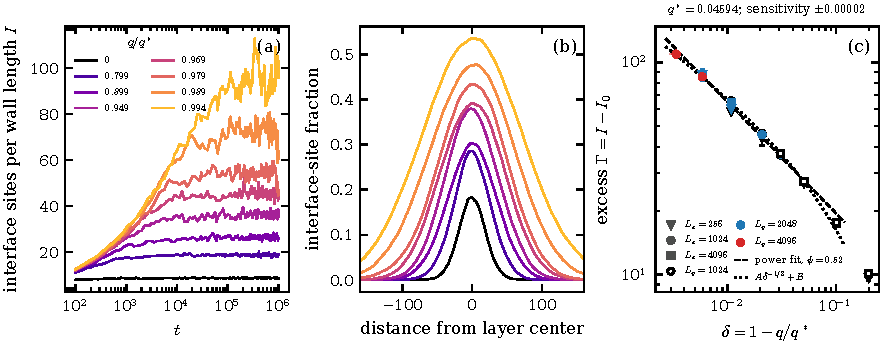
\includegraphics[width=\textwidth]{figs/fig_wall05}
\caption{Wetting at $p=1/2$, referenced to $q^*=0.04592$.
(a) Interface sites per unit wall length against time for $L_x=L_y=1024$
(four seeds per curve). (b) Interface-site fraction across the layer, centered
on its interface-weighted mean row before averaging late records.
(c) Excess adsorption for several box sizes (two to four seeds per point);
vertical bars show standard errors over runs including baseline uncertainty.
Horizontal bars on the fit points show the effect of varying $q^*$ by
$\pm0.00002$, a systematic sensitivity range. The dashed pure-power fit and
dotted $A\delta^{-1/3}+B$ fit use the same seven points with $L_x=1024$,
$L_y\ge2048$ and $\delta\le0.1$. The latter describes these data within their
sampling errors; neither fit determines the asymptotic law.}
\label{fig:wall}
\end{figure*}

